% Options for packages loaded elsewhere
\PassOptionsToPackage{unicode}{hyperref}
\PassOptionsToPackage{hyphens}{url}
\PassOptionsToPackage{dvipsnames,svgnames,x11names}{xcolor}
%
\documentclass[
  letterpaper,
  DIV=11,
  numbers=noendperiod]{scrartcl}

\usepackage{amsmath,amssymb}
\usepackage{iftex}
\ifPDFTeX
  \usepackage[T1]{fontenc}
  \usepackage[utf8]{inputenc}
  \usepackage{textcomp} % provide euro and other symbols
\else % if luatex or xetex
  \usepackage{unicode-math}
  \defaultfontfeatures{Scale=MatchLowercase}
  \defaultfontfeatures[\rmfamily]{Ligatures=TeX,Scale=1}
\fi
\usepackage{lmodern}
\ifPDFTeX\else  
    % xetex/luatex font selection
\fi
% Use upquote if available, for straight quotes in verbatim environments
\IfFileExists{upquote.sty}{\usepackage{upquote}}{}
\IfFileExists{microtype.sty}{% use microtype if available
  \usepackage[]{microtype}
  \UseMicrotypeSet[protrusion]{basicmath} % disable protrusion for tt fonts
}{}
\makeatletter
\@ifundefined{KOMAClassName}{% if non-KOMA class
  \IfFileExists{parskip.sty}{%
    \usepackage{parskip}
  }{% else
    \setlength{\parindent}{0pt}
    \setlength{\parskip}{6pt plus 2pt minus 1pt}}
}{% if KOMA class
  \KOMAoptions{parskip=half}}
\makeatother
\usepackage{xcolor}
\setlength{\emergencystretch}{3em} % prevent overfull lines
\setcounter{secnumdepth}{-\maxdimen} % remove section numbering
% Make \paragraph and \subparagraph free-standing
\ifx\paragraph\undefined\else
  \let\oldparagraph\paragraph
  \renewcommand{\paragraph}[1]{\oldparagraph{#1}\mbox{}}
\fi
\ifx\subparagraph\undefined\else
  \let\oldsubparagraph\subparagraph
  \renewcommand{\subparagraph}[1]{\oldsubparagraph{#1}\mbox{}}
\fi


\providecommand{\tightlist}{%
  \setlength{\itemsep}{0pt}\setlength{\parskip}{0pt}}\usepackage{longtable,booktabs,array}
\usepackage{calc} % for calculating minipage widths
% Correct order of tables after \paragraph or \subparagraph
\usepackage{etoolbox}
\makeatletter
\patchcmd\longtable{\par}{\if@noskipsec\mbox{}\fi\par}{}{}
\makeatother
% Allow footnotes in longtable head/foot
\IfFileExists{footnotehyper.sty}{\usepackage{footnotehyper}}{\usepackage{footnote}}
\makesavenoteenv{longtable}
\usepackage{graphicx}
\makeatletter
\def\maxwidth{\ifdim\Gin@nat@width>\linewidth\linewidth\else\Gin@nat@width\fi}
\def\maxheight{\ifdim\Gin@nat@height>\textheight\textheight\else\Gin@nat@height\fi}
\makeatother
% Scale images if necessary, so that they will not overflow the page
% margins by default, and it is still possible to overwrite the defaults
% using explicit options in \includegraphics[width, height, ...]{}
\setkeys{Gin}{width=\maxwidth,height=\maxheight,keepaspectratio}
% Set default figure placement to htbp
\makeatletter
\def\fps@figure{htbp}
\makeatother
% definitions for citeproc citations
\NewDocumentCommand\citeproctext{}{}
\NewDocumentCommand\citeproc{mm}{%
  \begingroup\def\citeproctext{#2}\cite{#1}\endgroup}
\makeatletter
 % allow citations to break across lines
 \let\@cite@ofmt\@firstofone
 % avoid brackets around text for \cite:
 \def\@biblabel#1{}
 \def\@cite#1#2{{#1\if@tempswa , #2\fi}}
\makeatother
\newlength{\cslhangindent}
\setlength{\cslhangindent}{1.5em}
\newlength{\csllabelwidth}
\setlength{\csllabelwidth}{3em}
\newenvironment{CSLReferences}[2] % #1 hanging-indent, #2 entry-spacing
 {\begin{list}{}{%
  \setlength{\itemindent}{0pt}
  \setlength{\leftmargin}{0pt}
  \setlength{\parsep}{0pt}
  % turn on hanging indent if param 1 is 1
  \ifodd #1
   \setlength{\leftmargin}{\cslhangindent}
   \setlength{\itemindent}{-1\cslhangindent}
  \fi
  % set entry spacing
  \setlength{\itemsep}{#2\baselineskip}}}
 {\end{list}}
\usepackage{calc}
\newcommand{\CSLBlock}[1]{\hfill\break\parbox[t]{\linewidth}{\strut\ignorespaces#1\strut}}
\newcommand{\CSLLeftMargin}[1]{\parbox[t]{\csllabelwidth}{\strut#1\strut}}
\newcommand{\CSLRightInline}[1]{\parbox[t]{\linewidth - \csllabelwidth}{\strut#1\strut}}
\newcommand{\CSLIndent}[1]{\hspace{\cslhangindent}#1}

\KOMAoption{captions}{tableheading}
\makeatletter
\@ifpackageloaded{caption}{}{\usepackage{caption}}
\AtBeginDocument{%
\ifdefined\contentsname
  \renewcommand*\contentsname{Table of contents}
\else
  \newcommand\contentsname{Table of contents}
\fi
\ifdefined\listfigurename
  \renewcommand*\listfigurename{List of Figures}
\else
  \newcommand\listfigurename{List of Figures}
\fi
\ifdefined\listtablename
  \renewcommand*\listtablename{List of Tables}
\else
  \newcommand\listtablename{List of Tables}
\fi
\ifdefined\figurename
  \renewcommand*\figurename{Figure}
\else
  \newcommand\figurename{Figure}
\fi
\ifdefined\tablename
  \renewcommand*\tablename{Table}
\else
  \newcommand\tablename{Table}
\fi
}
\@ifpackageloaded{float}{}{\usepackage{float}}
\floatstyle{ruled}
\@ifundefined{c@chapter}{\newfloat{codelisting}{h}{lop}}{\newfloat{codelisting}{h}{lop}[chapter]}
\floatname{codelisting}{Listing}
\newcommand*\listoflistings{\listof{codelisting}{List of Listings}}
\makeatother
\makeatletter
\makeatother
\makeatletter
\@ifpackageloaded{caption}{}{\usepackage{caption}}
\@ifpackageloaded{subcaption}{}{\usepackage{subcaption}}
\makeatother
\ifLuaTeX
  \usepackage{selnolig}  % disable illegal ligatures
\fi
\usepackage{bookmark}

\IfFileExists{xurl.sty}{\usepackage{xurl}}{} % add URL line breaks if available
\urlstyle{same} % disable monospaced font for URLs
\hypersetup{
  pdfauthor={Equipo EDUMER},
  colorlinks=true,
  linkcolor={blue},
  filecolor={Maroon},
  citecolor={Blue},
  urlcolor={Blue},
  pdfcreator={LaTeX via pandoc}}

\author{}
\date{}

\begin{document}

\section{The socialization of meritocracy and market justice preferences
at
school}\label{the-socialization-of-meritocracy-and-market-justice-preferences-at-school}

\subsection{Introduction}\label{introduction}

Since its origins, educational institutions have been related to the
idea of social mobility and access to better opportunities. Therefore,
the consistent evidence of the high level of social reproduction at the
school level represents a threat to the promise of education and a
meritocratic system (\citeproc{ref-bourdieu_reproduction_1990}{Bourdieu
and Passeron 1990}). A large part of the research in this field at an
international level has addressed the extent to which the social origin
of students affects their academic results and their life opportunities
(\citeproc{ref-vonhippel_test_2019}{Von Hippel and Hamrock 2019}),
confirming that schools have severe difficulties in closing the gaps of
origin. Besides this socioeconomic perspective on school opportunities,
recent research has addressed to what extent inequalities in the school
context are also influencing students' perceptions, beliefs, and
attitudes: Are social inequalities perceived at the school context? Are
they rejected by the students, particularly those who are worst-off in
socioeconomic terms? Or, Is there evidence at the school level that
social inequalities are tolerated and even justified?
(\citeproc{ref-batruch_belief_2022}{Batruch et al. 2022};
\citeproc{ref-wiederkehr_belief_2015}{Wiederkehr et al. 2015}).

In the present paper, we deal with the justification of social
inequalities by eighth-grade students in Chile, a country characterized
by a highly stratified educational system. In particular, we focus on
market justice preferences (\citeproc{ref-lane_market_1986}{Lane 1986}),
which refer to the preferences for distributing public goods (as health
and education) based on criteria such as competition and payment
capacity. Although from a rational point of view it could be expected an
opposition to market justice by the underprivileged majority, we argue
that in a social environment characterized by a promotion of
meritocratic ideals - as the school system - would lead to the opposite:
a larger market justice preferences.

Given that the school environment has an important focus on performance,
achievement and acknowledgment, meritocracy has been one of the
principal concepts used for understanding and even for justifying
performance differences among students. Meritocracy is a distributive
system based on the belief that people should be rewarded and promoted
based on their abilities, knowledge, and achievements
(\citeproc{ref-young_rise_1958}{Young 1958}). It is often seen as a way
to create equal opportunities and fairness, as individuals can rise to
positions of power and influence based on their own merit rather than
their background or connections. However, some argue that meritocracy
can actually lead to tolerating or even justifying social inequalities,
as it can create a hierarchy where those who already have resources and
advantages are more likely to succeed. In this regard, a great deal of
academic research about meritocracy delves into the assessment of to
what extent rewards and privileges in society are related to merit,
emphasizing the so-called unfulfillable promise of meritocracy
(\citeproc{ref-mijs_stratified_2016}{Mijs 2016}). Complementing this
agenda, a second and emerging research area deals with subjective
aspects of meritocracy, such as perceptions and beliefs.

{[}definición de market justice, welfare marketization, (Lindh){]}

{[}contexto Chileno market justice, dar cifras/porcentajes de
privatización de salud, educación y pensiones; asociar al tema de la
calidad (lo público es peor){]}

The perception of meritocracy refers to how individuals view and
understand the concept of meritocracy in their own society
(\citeproc{ref-duru-bellat_who_2012}{Duru-Bellat and Tenret 2012};
\citeproc{ref-castillo_meritocracia_2019}{Castillo et al. 2019}). This
perception can vary greatly depending on individual experiences, social,
economic, and cultural background. Some people may see meritocracy as a
fair and just system that allows anyone to succeed based on their
abilities and hard work. In contrast, others may view it as a myth or a
cover for existing power dynamics and inequality, serving to maintain
and even reinforce inequality
(\citeproc{ref-lampert_meritocratic_2013}{Lampert 2013};
\citeproc{ref-mijs_paradox_2021}{Mijs 2021}). Based in this last
perspective, we argue that individuals with a higher perception of
meritocracy will show a larger justification of social inequalities, as
individual achievement would be seen as rewarded and social policies as
less necessary (\citeproc{ref-batruch_belief_2022}{Batruch et al.
2022}).

Most of the research that has related meritocratic beliefs to inequality
justification so far has only considered adults, leaving aside the study
of how beliefs in this field develop at student age as well as the
impact of the school context and the family as the main socialization
agencies. Regarding schools, the way in which they deal with unequal
conditions of origin has been linked to the \emph{hidden curriculum}
(\citeproc{ref-chafel_schooling_1997}{Chafel 1997}), whereby students
learn about distributive norms in society and mechanisms of
justification of social differences. Based on recent studies that relate
school meritocracy to the justification of economic inequalities in the
adult population (\citeproc{ref-batruch_belief_2022}{Batruch et al.
2022}; \citeproc{ref-wiederkehr_belief_2015}{Wiederkehr et al. 2015}),
the central hypothesis guiding this research is that school-age students
with a higher perception of meritocracy - both at school and at the
societal level - will show a larger justification of social
inequalities, as individual achievement would be seen as appropriately
rewarded and social mechanisms for correcting inequalities as less
necessary (\citeproc{ref-batruch_belief_2022}{Batruch et al. 2022}).

\textasciitilde{}

{[}introducir distinción sobre percepción de meritocracia a nivel
escolar y a nivel de la sociedad{]}

{[}resaltar 3 focos de innovación: market justice preferences at school
level, relación con meritocracia, y esquema de meritocracia en la
escuela y en la sociedad{]}

The present paper deals with the association between the perception of
meritocracy and the justification of social inequalities, with two main
focuses. Firstly, it assesses the justification of social inequalities
in social policy domains, such as health, pensions, and education. We
argue that individuals who perceive more meritocracy would be more
willing to justify better services in these domains for those with
higher incomes. Secondly, we focus on the student-age population as we
point out that it is possible to track down the origin of meritocratic
beliefs (and their consequences) to early socialization processes. To
this regard, we take into account the family and the school as two main
socialization agencies that play a significant role in the socialization
of cultural beliefs by transmitting cultural norms, values, and
expectations to young people.

\subsection{Justification of
inequality}\label{justification-of-inequality}

Research on social stratification beliefs, which explore individual
perceptions of who deserves what and why
(\citeproc{ref-kluegel_beliefs_1987}{Kluegel and Smith 1987}),
highlights that people's explanations and justifications of social
inequality are closely tied to their judgments of deservingness. The
influence of ideologies (\citeproc{ref-wegener_dominant_1995}{Wegener
and Liebig 1995}) and cultural schemas
(\citeproc{ref-homan_being_2017}{Homan, Valentino, and Weed 2017}) is
pivotal in shaping these explanations by offering symbolic
representations that frame societal structures and expectations. While
significant attention has been paid to wage inequality, income
distribution, and payment differentials in the literature {[}Castillo
(\citeproc{ref-castillo_legitimacy_2011}{2011}); Evans et al., 2010;
Jasso (\citeproc{ref-jasso_how_1999}{1999}) ; Shariff, Wiwad, and Aknin
(\citeproc{ref-shariff_income_2016}{2016}){]}, there has been less
examination of public beliefs about which life domains should be
governed by market relations and even less about children's acceptance
or rejection of these market principles. This oversight is notable given
the extensive encroachment of market logic into public goods, welfare
policy, and social services over the past five decades
(\citeproc{ref-centeno_arc_2012}{Centeno and Cohen 2012};
\citeproc{ref-harvey_breve_2015}{Harvey 2015}), affecting areas such as
pensions, health services, and education. The justification of social
inequality based on marketype criteria has been conceptualized as the
individuals' adherence to one specific justice evaluation, the market
justice, that is, affording legitimacy to the allocation of goods and
services based on prices and individuals' ability to pay
(\citeproc{ref-boltanski_new_2005}{Boltanski and Chiapello 2005};
\citeproc{ref-lane_market_1986}{Lane 1986};
\citeproc{ref-streeck_citizens_2012}{Streeck 2012}).

Robert E. Lane proposed the underpinnings of market justice, which he
differentiated from political justice. For him, ``it is the genius of
the market to stimulate wants without at the same time stimulating a
sense of deserving more than one gets'' {[}-Lane
(\citeproc{ref-lane_market_1986}{1986}); p.~384{]}. Following the theory
of relative deprivation --a social phenomenon arising when individuals
cannot afford what most others in their environment can (Merton 1950)--
Lane notes that, in market settings, social comparisons are more likely
to motivate increased effort rather than feelings of acute injustice
because individuals attribute outcomes to their actions. Although
empirical research has shown that, contrary to Lane's observation,
relative deprivation, even in market settings, produces feelings of
dissatisfaction, anger, and resentment that might motivate forms of
collective action such as protests and revolt
(\citeproc{ref-greitemeyer_subjective_2016}{Greitemeyer and Sagioglou
2016}; \citeproc{ref-mishra_subjective_2015}{Mishra and Carleton 2015};
\citeproc{ref-smith_relative_2012}{Smith et al. 2012};
\citeproc{ref-power_deprivationprotest_2018}{Séamus A. Power 2018};
\citeproc{ref-power_relative_2020}{Séamus A. Power, Madsen, and Morton
2020}), the conceptualization of market justice has been since then
closely coupled to the merit principle for allocating outcomes: the
claim that the unequal levels of well-being individuals enjoy ought to
be, to some extent, a function of their talents and efforts, regardless
of their needs or membership, the two latter being the realm of
political justice and its closely coupled principles of need
--allocating outcomes to those who require them most-- and equality
--allocating the same outcome to everyone--, which have been at the
center of welfarism (see Wilson 2003). The underlying notion of market
justice also resonates in its application to welfare regimes, providing
a framework for understanding the varied global approaches to managing
social services.

The management of social services manifests in varying approaches across
nations, with substantial differences in funding and delivery methods
(\citeproc{ref-jensen_worlds_2008}{Jensen 2008};
\citeproc{ref-stoy_worlds_2014}{Stoy 2014}). Nordic countries, for
example, predominantly employ public agencies to produce and provide
social services, funding these through collective taxation and offering
them in kind to the majority of citizens. This system prioritizes
political justice, placing it above market mechanisms in accessing
services. In contrast, other countries rely more heavily on for-profit
entities and private funding, where service distribution depends mainly
on individual financial capacity of paying user fees, highlighting the
influence of market justice in service allocation. The trend toward
marketization of welfare services has been growing since the 1980s
(\citeproc{ref-salamon_marketization_1993}{Salamon 1993}), and this
shift is increasingly evident even in countries where market solutions
have traditionally had a minor role in social policy
(\citeproc{ref-sivesind_changing_2017}{Sivesind 2017}).

The question arises whether adults and children justify unequal access
to welfare services based on market justice principles. Influenced by
theories of policy feedback, which suggest that social welfare policies
can reinforce (positive feedback) or undermine (negative feedback)
previous policy trajectories
(\citeproc{ref-fernandez_positive_2013}{Fernandez and Jaime-Castillo
2013}; \citeproc{ref-pierson_increasing_2000}{Pierson 2000};
\citeproc{ref-weaver_paths_2010}{Weaver 2010}), citizens' beliefs about
market justice are likely also shaped by the institutional and social
contexts they encounter. Indeed, the justification of inequality in
access to essential services like education and health, based on one's
ability to pay, shows significant variation across countries, as
demonstrated by international surveys, although they do not usually
include children in their samples. For instance, the 2019 International
Social Survey Program (ISSP) provides insights into how adults perceive
inequality in accessing welfare services. Figure~\ref{fig-issp}
illustrates the variation in agreement levels regarding whether it is
just for individuals with higher incomes to purchase better education or
healthcare. Notably, in 18 of the 29 countries analyzed, there is a
greater justification for market inequality in healthcare access than in
education. Nevertheless, the general sentiment typically ranges from
`somewhat unjust' to 'neither just nor unjust, with mixed feelings.

\begin{figure}

\centering{

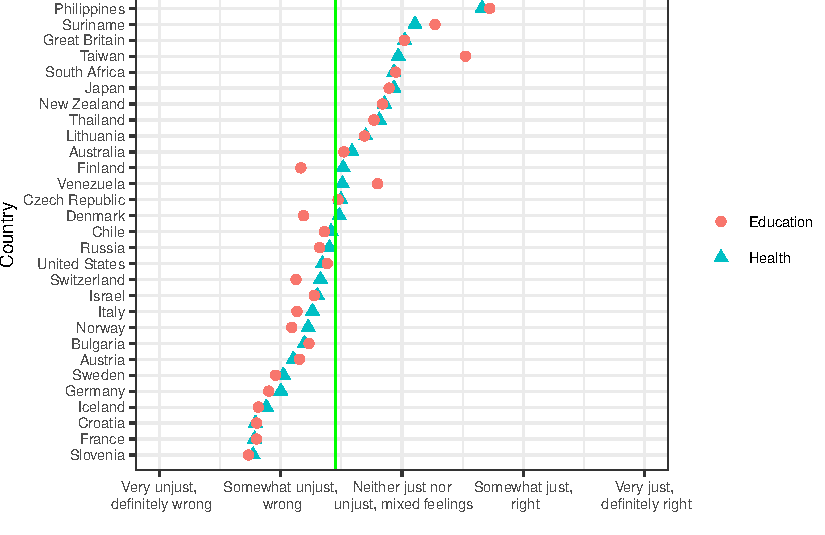
\includegraphics{paper_files/figure-pdf/fig-issp-1.pdf}

}

\caption{\label{fig-issp}Average of market justice preferences by
country}

\end{figure}%

While contemporary policy developments have increasingly embraced the
marketization of social welfare in areas such as education, pensions,
and health services, questions about public acceptance of these changes
persist. Lindh (\citeproc{ref-lindh_public_2015}{2015}) analysis of ISSP
2009 data from 17 OECD countries reveals a general lack of support for
market-based distribution of social services, suggesting widespread
disapproval of market stratification of essential services. This finding
is corroborated by Soler-Martínez, García-Sánchez, and Willis
(\citeproc{ref-soler-martinez_concerns_2023}{2023}) research from
Latinobarómetro 2020 across 18 Latin American countries, where concerns
about health and education access predominated over income inequality.
These results indicate that reforms toward welfare marketization are
typically driven by elite political decisions rather than grassroots
demand.

Despite high-income inequality and limited social mobility in Latin
America, there is a prevalent belief that individuals are solely
responsible for their economic outcomes, a view that varies across the
region (\citeproc{ref-bucca_merit_2016}{Bucca 2016};
\citeproc{ref-chong_mystery_2008}{Chong and Ñopo 2008};
\citeproc{ref-torche_intergenerational_2014}{Torche 2014};
\citeproc{ref-salgado_inequality_2023}{Salgado and Castillo 2023}). The
reliance on private welfare providers and widespread user fees
(\citeproc{ref-molyneux_neoliberal_2008}{Molyneux 2008}) adds complexity
to this context. Yet, research on children's justification of
market-based inequalities in accessing welfare services remains limited,
especially in Latin America, highlighting a significant gap in
understanding how younger generations view market-based access to
welfare and whether these views are associated with their meritocratic
beliefs.

\subsection{Meritocracy}\label{meritocracy}

The concept of meritocracy frequently appears nowadays when analyzing
cultural determinants of social inequalities. In general, it is
mentioned as a value associated with justice, as it would link efforts
and talents with rewards in an equitable manner. This normative sense is
quite far from its original formulation by Young
(\citeproc{ref-young_rise_1958}{1958}) in the satirical novel ``The Rise
of Meritocracy'', where it ironically represented a mechanism for
reproducing the inequalities of origin. The meritocratic ideal had
remained relatively unchallenged until a series of recent publications
turned into its potential consequences for maintaining social
inequality. Perhaps one of the most recent sources in this line is
Michael Sandel's ``The Tyranny of Merit'', where he strongly questions
the implications of carrying out the principle of merit in societies
that do not guarantee equal opportunities and that generate a feeling of
scarce recognition and appreciation of those who receive lesser rewards:
``In society's eyes, and perhaps also their own, their work no longer
signified a valued contribution to the common good.''
(\citeproc{ref-sandel_tyranny_2020}{Sandel 2020}, pp.).

Empirical research on meritocracy has increased along with the
philosophical-normative discussion on meritocracy in recent years.
Particularly from a sociological perspective, meritocracy has been used
in research on social mobility to characterize societies with low
mobility that threaten the meritocratic ideal
(\citeproc{ref-goldthorpe_myth_2003}{Goldthorpe 2003}). More recently,
sociology and social psychology research has attended to the subjective
aspects vis-a-vis beliefs in meritocracy. The label of beliefs in this
realm covers a series of areas, such as attitudes, perceptions, and
preferences (Castillo et al), whereby most of the link this subjective
dimensions to individual socio-structural factors and context-level
determinants. For instance, some studies have analyzed how those with
greater privileges believe more in meritocracy (Reynolds \& Chan 2014),
how greater economic inequality increases meritocratic beliefs
(\citeproc{ref-mijs_paradox_2021}{Mijs 2021}), and how larger inequality
affects meritocratic beliefs
(\citeproc{ref-morris_representing_2022}{Morris et al. 2022}). Based on
these findings, a research agenda has been reinforced on the
legitimizing role of meritocracy, in line with previous studies using
the concept of a just world (Lerner, Dalbert) and the theory of system
justification (Jost \& Major).

How do meritocratic beliefs legitimize inequalities? Empirical studies
have used experiments and surveys to address this question. For
instance, the evidence suggests that just world beliefs correlate
negatively with support for redistributive compensation systems
(\citeproc{ref-frank_performance_2015}{Frank, Wertenbroch, and Maddux
2015}). Conversely, individuals tend to support redistribution when they
believe that the disadvantaged lack the opportunities to succeed
(\citeproc{ref-evans_strong_2018}{Evans and Kelley 2018}). Almås,
Cappelen, and Tungodden (\citeproc{ref-almas_cutthroat_2020}{2020})
found that in a relatively unequal society (the United States), the
highly educated accept inequality significantly more than the less
educated because they perceive inequality as justifiable owing to
differences in productivity (i.e., merit), whereas in a relatively equal
society (Norway), the less educated accept inequality more, but not
significantly more than the highly educated because meritocratic values
are less prevalent. Barr and Miller
(\citeproc{ref-barr_effect_2020}{2020}) also addressed this triple
interaction between the level of inequality in a society, the individual
level of education, and the perceived origin of the disparity (either by
luck or effort) to determine the extent to which inequality is accepted.
They found that the interaction's mechanism varies depending on the
compared societies. Finally, García-Sánchez et al.
(\citeproc{ref-garcia-sanchez_attitudes_2020}{2020}), using data for 41
countries from the International Social Survey Programme (ISSP), found
that the perceived size of the income gap correlated positively with
support for progressive taxation. Still, this association was weaker
among those who endorsed meritocratic and equal opportunity beliefs. In
the same line, experimental research by Durante and Putterman
(\citeproc{ref-durante_preferences_2009}{2009}) subjects support less
redistribution when the initial distribution is determined according to
task performance.

Research about meritocratic beliefs at school age is rather scarce,
leaving a wide research gap as schools are one of the primary
socialization institutions where achievement based on merit explains
success (\citeproc{ref-erivwo_meritocracy_2021}{Erivwo et al. 2021}).
Nevertheless, it is possible to find some initial works focused on the
area of distributive justice at school that are closely related to
meritocratic beliefs, as the ones by Resh and Sabbagh (quotes). Using
justice in grade obtention as a measure of distributive justice and
meritocracy (Sabbagh et al 2006), they find for instance that a larger
sense of distributive justice about grades is associated to higher
socio-economic status (\citeproc{ref-resh_sense_2010}{Resh 2010}), have
a positive effect on liberal democratic orientation and on trust in
people and in formal institutions (\citeproc{ref-resh_sense_2014}{Resh
and Sabbagh 2014}), and tend to refrain from violence and to engage to a
greater extent in extra-curricular school activity and community
volunteering (\citeproc{ref-resh_sense_2017}{Resh and Sabbagh 2017}).

\subsection{Children's judgments of inequality, schools, and family
background}\label{childrens-judgments-of-inequality-schools-and-family-background}

Research indicates various socialization practices at families and
schools during childhood and adolescence that impact dispositional and
behavioral tendencies concerning justifications of inequality in adult
life. The differences in economic understanding across age groups are
consistent with research on cognitive development
(\citeproc{ref-choudhury_social_2006}{Choudhury, Blakemore, and Charman
2006}). Adolescents with mature socio-cognitive abilities tend to
express stronger preferences for fairness than infants and children
(\citeproc{ref-wynn_not_2018}{Wynn et al. 2018}). As children grow
older, they become more likely to behave fairly, with their
early-emerging strict egalitarianism being replaced by an increasing
endorsement of fairness principles and engagement in collaborative
activities (\citeproc{ref-huppert_development_2019}{Huppert et al.
2019}; \citeproc{ref-mcauliffe_developmental_2017}{McAuliffe et al.
2017}). In these activities, their fairness views consider individual
contributions, merits, and circumstances
(\citeproc{ref-almas_fairness_2010}{Almås et al. 2010};
\citeproc{ref-huppert_development_2019}{Huppert et al. 2019};
\citeproc{ref-sigelman_development_1991}{Sigelman and Waitzman 1991}).
Engelmann and Tomasello (\citeproc{ref-engelmann_children_2019}{2019})
claim that children's sense of fairness emerges at three years old, and
we can observe it in collaborative activities, where they accept
inequality if the procedure gives everyone an equal chance. Therefore,
children at this age respond to unequal distributions based on
interpersonal concerns, as they already demand equal respect. In any
case, between 3 and 8 years of age, inequitable and anti-meritorious
allocations are evaluated more negatively, but equitable and meritorious
allocations are not evaluated more positively
(\citeproc{ref-elenbaas_unfairness_2019}{Elenbaas 2019}).

Some research shows that the social environment in which children
develop, such as family and school, is associated with their prosocial
behaviors by playing an essential role in the transmission of equity
norms (\citeproc{ref-schunk_fairness_2023}{Schunk and Zipperle 2023};
\citeproc{ref-kosse_prosociality_2020}{Kosse and Tincani 2020}). In
fact, schools contribute to institutionalizing and reproducing
inequality by promoting values, norms, practices, and languages familiar
to higher-class families because the dominant group's culture shapes
educational institutions
(\citeproc{ref-bourdieu_reproduction_1990}{Bourdieu and Passeron 1990}).
Middle- and upper-class students are better equipped to face academic
challenges and are more familiar with academic expectations
(\citeproc{ref-mikus_children_2020}{Mikus, Tieben, and Schober 2020}).
Such familiarity represents cultural capital in educational contexts
because higher-status students come to school ready to meet these
expectations and reap the benefits (\citeproc{ref-jack_no_2016}{Jack
2016}; \citeproc{ref-khan_privilege_2011}{Khan 2011}). Conversely,
lower-status children lacking cultural capital must catch up while
experiencing inequitable comparisons
(\citeproc{ref-goudeau_hidden_2017}{Goudeau and Croizet 2017}).
Additionally, academic achievement is treated as the outcome of
dispositional factors (e.g., pupils' efforts and talents or lack of
them) rather than the result of differential access to critical
resources. Due to the meritocratic frame schools encourage, both low-
and high-status individuals believe that students' success or failure is
not due to their family background but rather to differences in efforts
and talents (\citeproc{ref-darnon_where_2018}{Darnon et al. 2018}). In
this sense, we believe that the perception of meritocracy can influence
students' judgments about market justice preferences. Furthermore, we
believe there is a difference between students' perceptions of
meritocracy based on their own experience in school and what they
perceive in society at large. Consistently, our first two hypotheses
are:

H1a: Students who perceive that there is more meritocracy at school will
show larger market justice preferences

H1b: Students who perceive that there is more meritocracy in society
will show larger market justice preferences

Family background and family socialization practices also contribute to
children's and adolescent's market justice preferences. For example,
Almås et al. (\citeproc{ref-almas_fairness_2017}{2017}) found that
adolescents from low-socioeconomic-status families are likelier to have
an egalitarian fairness view and consider an equal distribution as fair
in a situation with unequal merits. The authors speculate that
differences in socialization practices across status groups might bring
about, to a great extent, the fairness views of children and adolescents
because social status seems to interact with these evaluations (e.g.,
\citeproc{ref-hvidberg_social_2023}{Hvidberg, Kreiner, and Stantcheva
2023}).

The classic work of Kohn showed that middle-class parents value the
expression of internal states and emotions, such as self-control,
curiosity, happiness, and consideration, while working-class parents
promote deference, obedience, and conformity to authority
(\citeproc{ref-kohn_social_1963}{Kohn 1963};
\citeproc{ref-kohn_class_1969}{Kohn and Schooler 1969}). Although
parents from all social backgrounds encourage individualism in their
children, this shared norm translates into different forms in high and
low social classes (1999). Acemoglu
(\citeproc{ref-acemoglu_obedience_2021}{2021}) claimed that the values
families impart to their children interact with social mobility. Because
obedience is a valuable characteristic for employers, in low-wage and
social mobility environments, low-income families impart values of
obedience to their children to prevent disadvantaging them in labor
markets. On the one hand, children from privileged families are
socialized to adopt a clear conception of individualism that highlights
their internal states, independence, and idiosyncrasies. In contrast,
children from disadvantaged families are socialized to support a more
balanced view of individualism that considers personal characteristics
as resources to overcome collective impediments on the path to upward
mobility (\citeproc{ref-iacoviello_collectivism_2019}{Iacoviello and
Lorenzi-Cioldi 2019}). In this way, we believe that there are
differences in the socialization of values according to socioeconomic
differences that could influence market justice preferences and,
therefore, we propose the following hypothesis:

H2: Students from families of higher social status will show larger
market justice preferences.

Recent empirical research has demonstrated that the institutional design
of schools, coupled with the meritocratic ideology it fosters,
significantly influences children's and adolescents' views on inequality
and deservingness. For example, Jonsson and Beach
(\citeproc{ref-jonsson_institutional_2015}{2015}) study revealed that
higher-status adolescents in Sweden tend to perpetuate social class
stereotypes while describing the vocational and academic tracks.
Academic track students are depicted as wealthy, intelligent, ambitious,
and diligent, while vocational track students are characterized as poor,
unambitious, unintelligent, and lackadaisical. These stereotypes help
individuals maintain a sense of superiority over others and legitimize
the prevailing social hierarchies and economic disparities
(\citeproc{ref-jost_attitudinal_2000}{Jost and Burgess 2000})

H3: Students from schools of higher social status will show larger
market justice preferences.

H4: Students from schools with higher average levels of academic
achievement will show larger market justice preferences.

{[}interacciones{]}

H5: The perception of meritocracy in school and society will moderate
the effect of family social status on market justice preferences.

H6: The perception of meritocracy in school and society will moderate
the effect of school status on market justice preferences.

H7: The perception of meritocracy in school and society will moderate
the effect of school academic achievement on market justice preferences.

\subsubsection{Summary of hypotheses}\label{summary-of-hypotheses}

\begin{figure}

\centering{

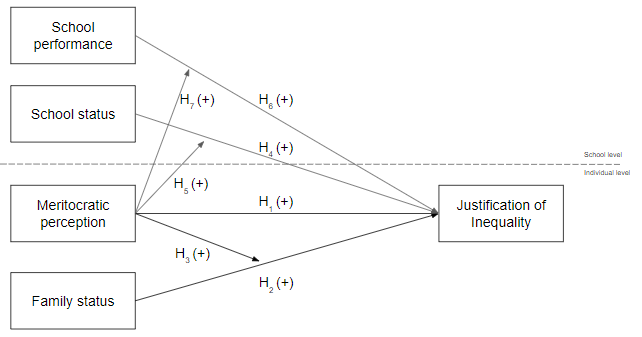
\includegraphics{input/img/hypotheses.png}

}

\caption{\label{fig-hypotheses}Summary of hypotheses}

\end{figure}%

\subsection{}\label{section}

\subsection{Methods}\label{methods}

\subsubsection{Data}\label{data}

The main data source for the analysis is the First Study of Citizenship
Education in Chile, carried out by the Education Quality Agency of the
Ministry of Education. The application date was November 9, 2017. The
target population of this study is Eighth-grade students from 242
schools. In the data, there are 8,589 students and 6,770 parents. This
database was analyzed with the R package ``ResponsePatterns'' to detect
possible repetitive and ``careless'' response patterns and thus
contribute to a higher quality of research data (Gottfried, et al 2022).
Responses from 171 students and 79 parents were removed, which, when
merged, gave a total of 6,270 valid cases.

The analysis of school variables includes data from the Ministry of
Education's SIMCE 2017 database. This database contains information at
the school level, such as the administrative dependency, its
socioeconomic classification, and the achievement scores obtained in the
mathematics and language census tests. It is available for free use on
the MINEDUC {[}web page{]}.

After eliminating missing cases, the final sample used in the analysis
was based on 5,047 students and parents of 231 schools for the dependent
variable of access to social services.

\subsubsection{Variables}\label{variables}

\textbf{Dependent variables}

This study has three dependent variables related to the justification of
social inequality in specific policy domains. The first asks whether
access to social services should be conditional on income, i,.e., ``It
is just that in Chile people who can pay have a better education for
their children''. Students rated their preferences using the following
responses: ``strongly disagree'', ``Disagree'', ``Agree'', and
''strongly agree''. An average index is built with these items
(Cronbach's Alpha = 0,86). (Apéndice: items en español y su
correspondiente traducción al inglés)

Table~\ref{tbl-desc-dependientes} shows the items used, their response
categories, and their frequencies.

\begin{longtable}[]{@{}
  >{\raggedright\arraybackslash}p{(\columnwidth - 6\tabcolsep) * \real{0.4286}}
  >{\raggedright\arraybackslash}p{(\columnwidth - 6\tabcolsep) * \real{0.2551}}
  >{\raggedright\arraybackslash}p{(\columnwidth - 6\tabcolsep) * \real{0.2143}}
  >{\raggedright\arraybackslash}p{(\columnwidth - 6\tabcolsep) * \real{0.1020}}@{}}
\caption{Dependent
variables}\label{tbl-desc-dependientes}\tabularnewline
\toprule\noalign{}
\begin{minipage}[b]{\linewidth}\raggedright
Label
\end{minipage} & \begin{minipage}[b]{\linewidth}\raggedright
Stats / Values
\end{minipage} & \begin{minipage}[b]{\linewidth}\raggedright
Freqs (\% of Valid)
\end{minipage} & \begin{minipage}[b]{\linewidth}\raggedright
Valid
\end{minipage} \\
\midrule\noalign{}
\endfirsthead
\toprule\noalign{}
\begin{minipage}[b]{\linewidth}\raggedright
Label
\end{minipage} & \begin{minipage}[b]{\linewidth}\raggedright
Stats / Values
\end{minipage} & \begin{minipage}[b]{\linewidth}\raggedright
Freqs (\% of Valid)
\end{minipage} & \begin{minipage}[b]{\linewidth}\raggedright
Valid
\end{minipage} \\
\midrule\noalign{}
\endhead
\bottomrule\noalign{}
\endlastfoot
It is just that in Chile people with higher incomes can have better
pensions than people with low incomes &
\begin{minipage}[t]{\linewidth}\raggedright
1. Strongly disagree\\
2. Disagree\\
3. Agree\\
4. Strongly agree\strut
\end{minipage} & \begin{minipage}[t]{\linewidth}\raggedright
1837 (30.6\%)\\
1945 (32.4\%)\\
1622 (27.0\%)\\
608 (10.1\%)\strut
\end{minipage} & \begin{minipage}[t]{\linewidth}\raggedright
6012\\
(95.9\%)\strut
\end{minipage} \\
It is just that in Chile people who can pay have a better education for
their children & \begin{minipage}[t]{\linewidth}\raggedright
1. Strongly disagree\\
2. Disagree\\
3. Agree\\
4. Strongly agree\strut
\end{minipage} & \begin{minipage}[t]{\linewidth}\raggedright
1766 (29.7\%)\\
1732 (29.1\%)\\
1704 (28.6\%)\\
750 (12.6\%)\strut
\end{minipage} & \begin{minipage}[t]{\linewidth}\raggedright
5952\\
(94.9\%)\strut
\end{minipage} \\
It is just that in Chile people with higher incomes can access better
health services than people with low incomes &
\begin{minipage}[t]{\linewidth}\raggedright
1. Strongly disagree\\
2. Disagree\\
3. Agree\\
4. Strongly agree\strut
\end{minipage} & \begin{minipage}[t]{\linewidth}\raggedright
2254 (38.0\%)\\
1685 (28.4\%)\\
1401 (23.6\%)\\
593 (10.0\%)\strut
\end{minipage} & \begin{minipage}[t]{\linewidth}\raggedright
5933\\
(94.6\%)\strut
\end{minipage} \\
Inequality justification index &
\begin{minipage}[t]{\linewidth}\raggedright
Mean (sd) : 2.2 (0.9)\\
min \textless{} med \textless{} max:\\
1 \textless{} 2 \textless{} 4\\
IQR (CV) : 1.7 (0.4)\strut
\end{minipage} & 13 distinct values &
\begin{minipage}[t]{\linewidth}\raggedright
6077\\
(96.9\%)\strut
\end{minipage} \\
\end{longtable}

\textbf{Independent variables}

For the primary independent variable, the perception of meritocracy,
five items address the perception of rewards according to effort and
intelligence at the school and societal levels. At the school level,
students answer whether ``Intelligence is important to get good grades''
and ``Effort is important to get good grades''. At the societal level,
students respond to the following questions: ``In Chile, people are
rewarded for their efforts'', ``In Chile, people get what they
deserve'', and ``In Chile, people are rewarded for their intelligence
and skills''. Each item was answered on a four-point scale ranging from
``Strongly disagree'' to ``Strongly agree''.

The rest of the independent variables are divided into individual and
school levels. At the individual level, family socioeconomic status was
measured by the parents' highest educational level and the number of
books at home. Likewise, an index of access to technology includes the
number of computers, tablets, and cell phones at home, as well as
whether there is an Internet connection.
Table~\ref{tbl-desc-independent} shows the items used, their response
categories, and their frequency.

\begin{longtable}[]{@{}
  >{\raggedright\arraybackslash}p{(\columnwidth - 6\tabcolsep) * \real{0.3925}}
  >{\raggedright\arraybackslash}p{(\columnwidth - 6\tabcolsep) * \real{0.3084}}
  >{\raggedright\arraybackslash}p{(\columnwidth - 6\tabcolsep) * \real{0.1963}}
  >{\raggedright\arraybackslash}p{(\columnwidth - 6\tabcolsep) * \real{0.1028}}@{}}
\caption{Independent
variables}\label{tbl-desc-independent}\tabularnewline
\toprule\noalign{}
\begin{minipage}[b]{\linewidth}\raggedright
Label
\end{minipage} & \begin{minipage}[b]{\linewidth}\raggedright
Stats / Values
\end{minipage} & \begin{minipage}[b]{\linewidth}\raggedright
Freqs (\% of Valid)
\end{minipage} & \begin{minipage}[b]{\linewidth}\raggedright
Valid
\end{minipage} \\
\midrule\noalign{}
\endfirsthead
\toprule\noalign{}
\begin{minipage}[b]{\linewidth}\raggedright
Label
\end{minipage} & \begin{minipage}[b]{\linewidth}\raggedright
Stats / Values
\end{minipage} & \begin{minipage}[b]{\linewidth}\raggedright
Freqs (\% of Valid)
\end{minipage} & \begin{minipage}[b]{\linewidth}\raggedright
Valid
\end{minipage} \\
\midrule\noalign{}
\endhead
\bottomrule\noalign{}
\endlastfoot
Intelligence is important to get good grades &
\begin{minipage}[t]{\linewidth}\raggedright
1. Strongly disagree\\
2. Disagree\\
3. Agree\\
4. Strongly agree\strut
\end{minipage} & \begin{minipage}[t]{\linewidth}\raggedright
367 ( 6.1\%)\\
920 (15.3\%)\\
2970 (49.4\%)\\
1760 (29.3\%)\strut
\end{minipage} & \begin{minipage}[t]{\linewidth}\raggedright
6017\\
(95.9\%)\strut
\end{minipage} \\
Effort is important to get good grades &
\begin{minipage}[t]{\linewidth}\raggedright
1. Strongly disagree\\
2. Disagree\\
3. Agree\\
4. Strongly agree\strut
\end{minipage} & \begin{minipage}[t]{\linewidth}\raggedright
109 ( 1.8\%)\\
88 ( 1.5\%)\\
1427 (23.7\%)\\
4406 (73.1\%)\strut
\end{minipage} & \begin{minipage}[t]{\linewidth}\raggedright
6030\\
(96.1\%)\strut
\end{minipage} \\
In Chile, people are rewarded for their intelligence and skill &
\begin{minipage}[t]{\linewidth}\raggedright
1. Strongly disagree\\
2. Disagree\\
3. Agree\\
4. Strongly agree\strut
\end{minipage} & \begin{minipage}[t]{\linewidth}\raggedright
517 ( 9.0\%)\\
1568 (27.3\%)\\
2673 (46.6\%)\\
983 (17.1\%)\strut
\end{minipage} & \begin{minipage}[t]{\linewidth}\raggedright
5741\\
(91.5\%)\strut
\end{minipage} \\
In Chile, people are rewarded for their efforts &
\begin{minipage}[t]{\linewidth}\raggedright
1. Strongly disagree\\
2. Disagree\\
3. Agree\\
4. Strongly agree\strut
\end{minipage} & \begin{minipage}[t]{\linewidth}\raggedright
512 ( 8.7\%)\\
1733 (29.4\%)\\
2607 (44.2\%)\\
1050 (17.8\%)\strut
\end{minipage} & \begin{minipage}[t]{\linewidth}\raggedright
5902\\
(94.1\%)\strut
\end{minipage} \\
In Chile, people get what they deserve &
\begin{minipage}[t]{\linewidth}\raggedright
1. Strongly disagree\\
2. Disagree\\
3. Agree\\
4. Strongly agree\strut
\end{minipage} & \begin{minipage}[t]{\linewidth}\raggedright
604 (10.5\%)\\
1911 (33.1\%)\\
2388 (41.4\%)\\
871 (15.1\%)\strut
\end{minipage} & \begin{minipage}[t]{\linewidth}\raggedright
5774\\
(92.1\%)\strut
\end{minipage} \\
Parental educational level & \begin{minipage}[t]{\linewidth}\raggedright
1. 8th grade or less\\
2. Secondary Education\\
3. Higher tec. education\\
4. University or Postgraduat\\
5. Missing\strut
\end{minipage} & \begin{minipage}[t]{\linewidth}\raggedright
559 ( 8.9\%)\\
1698 (27.1\%)\\
960 (15.3\%)\\
1080 (17.2\%)\\
1975 (31.5\%)\strut
\end{minipage} & \begin{minipage}[t]{\linewidth}\raggedright
6272\\
(100.0\%)\strut
\end{minipage} \\
Number of books at home & \begin{minipage}[t]{\linewidth}\raggedright
1. Les than 25\\
2. More than 25\strut
\end{minipage} & \begin{minipage}[t]{\linewidth}\raggedright
3920 (63.2\%)\\
2281 (36.8\%)\strut
\end{minipage} & \begin{minipage}[t]{\linewidth}\raggedright
6201\\
(98.9\%)\strut
\end{minipage} \\
Technology access index & \begin{minipage}[t]{\linewidth}\raggedright
Mean (sd) : 7.8 (2.5)\\
min \textless{} med \textless{} max:\\
0 \textless{} 8 \textless{} 12\\
IQR (CV) : 3 (0.3)\strut
\end{minipage} & 13 distinct values &
\begin{minipage}[t]{\linewidth}\raggedright
6272\\
(100.0\%)\strut
\end{minipage} \\
\end{longtable}

The school-level variables are the administrative dependency of the
school, the socioeconomic classification made by the Ministry of
Education, the level of performance in the SIMCE test of the school, and
the proportion of parents with university or postgraduate degrees.
Table~\ref{tbl-desc-school} shows the items used, response categories,
and frequency.

\begin{longtable}[]{@{}
  >{\raggedright\arraybackslash}p{(\columnwidth - 6\tabcolsep) * \real{0.4040}}
  >{\raggedright\arraybackslash}p{(\columnwidth - 6\tabcolsep) * \real{0.2626}}
  >{\raggedright\arraybackslash}p{(\columnwidth - 6\tabcolsep) * \real{0.2222}}
  >{\raggedright\arraybackslash}p{(\columnwidth - 6\tabcolsep) * \real{0.1111}}@{}}
\caption{School context variables}\label{tbl-desc-school}\tabularnewline
\toprule\noalign{}
\begin{minipage}[b]{\linewidth}\raggedright
Label
\end{minipage} & \begin{minipage}[b]{\linewidth}\raggedright
Stats / Values
\end{minipage} & \begin{minipage}[b]{\linewidth}\raggedright
Freqs (\% of Valid)
\end{minipage} & \begin{minipage}[b]{\linewidth}\raggedright
Valid
\end{minipage} \\
\midrule\noalign{}
\endfirsthead
\toprule\noalign{}
\begin{minipage}[b]{\linewidth}\raggedright
Label
\end{minipage} & \begin{minipage}[b]{\linewidth}\raggedright
Stats / Values
\end{minipage} & \begin{minipage}[b]{\linewidth}\raggedright
Freqs (\% of Valid)
\end{minipage} & \begin{minipage}[b]{\linewidth}\raggedright
Valid
\end{minipage} \\
\midrule\noalign{}
\endhead
\bottomrule\noalign{}
\endlastfoot
Proportion of parents with university level by school &
\begin{minipage}[t]{\linewidth}\raggedright
Mean (sd) : 0.2 (0.2)\\
min \textless{} med \textless{} max:\\
0 \textless{} 0.1 \textless{} 0.9\\
IQR (CV) : 0.2 (0.9)\strut
\end{minipage} & 103 distinct values &
\begin{minipage}[t]{\linewidth}\raggedright
6272\\
(100.0\%)\strut
\end{minipage} \\
SIMCE score by school & \begin{minipage}[t]{\linewidth}\raggedright
1. Low\\
2. Medium\\
3. High\strut
\end{minipage} & \begin{minipage}[t]{\linewidth}\raggedright
2091 (33.3\%)\\
2091 (33.3\%)\\
2090 (33.3\%)\strut
\end{minipage} & \begin{minipage}[t]{\linewidth}\raggedright
6272\\
(100.0\%)\strut
\end{minipage} \\
Administrative dependency of school &
\begin{minipage}[t]{\linewidth}\raggedright
1. Public\\
2. Subsidized private\\
3. Private\strut
\end{minipage} & \begin{minipage}[t]{\linewidth}\raggedright
2659 (42.4\%)\\
3169 (50.5\%)\\
444 ( 7.1\%)\strut
\end{minipage} & \begin{minipage}[t]{\linewidth}\raggedright
6272\\
(100.0\%)\strut
\end{minipage} \\
Socioeconomic level of school &
\begin{minipage}[t]{\linewidth}\raggedright
1. Low\\
2. Medium low\\
3. Medium\\
4. Medium high\\
5. High\strut
\end{minipage} & \begin{minipage}[t]{\linewidth}\raggedright
720 (11.5\%)\\
2282 (36.4\%)\\
1383 (22.1\%)\\
1309 (20.9\%)\\
578 ( 9.2\%)\strut
\end{minipage} & \begin{minipage}[t]{\linewidth}\raggedright
6272\\
(100.0\%)\strut
\end{minipage} \\
\end{longtable}

\subsubsection{Methods}\label{methods-1}

The data has a hierarchical structure of students nested in schools, so
the model estimation is performed in a multilevel (random effects)
framework. This modeling approach lets us correctly estimate individual
and contextual effects in a single model. We estimate cumulative link
mixed models for the ordinal dependent variables, whereas we use linear
mixed effects models for the average index of inequality justification.

The hypotheses of this research were pre-registered in the Open Science
Framework platform of the Center for Open Science (OSF), the access to
the document is available at this
\href{https://doi.org/10.17605/OSF.IO/UFSDV}{link}. The statistical
analysis of this research was performed using the free software R
version 4.1.3.

\subsection{Analysis}\label{analysis}

\subsubsection{Descriptive analysis}\label{descriptive-analysis}

\begin{figure}[H]

{\centering 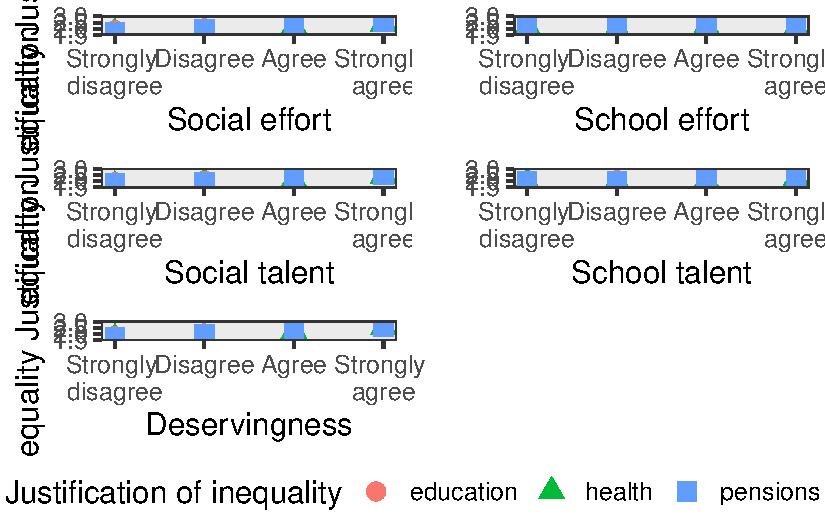
\includegraphics{paper_files/figure-pdf/unnamed-chunk-11-1.pdf}

}

\caption{Market justice preferences in education, health and pensions by
social and school meritocracy}

\end{figure}%

Figure 3 shows a series of graphs depicting the association between the
variables of market justice preferences - in education, health, and
pensions - and the variables of meritocratic perception at school
(effort and talent) and in society (effort, talent, and deservingness)
(see conceptual diagram en figure X). On the left, we observe the social
meritocracy diagrams, while on the right the school meritocracy diagrams
are shown. For the three variables of perception of meritocracy in
society the relationship is clear, since the average of market justice
preferences increases the more there is agreement that people are
rewarded for their effort, merit, and talent. This relationship needs to
be clarified in the case of the variables of perception of meritocracy
at school. To the extent that there is more agreement that the
perception of talent is essential for obtaining good grades, the average
of market justice preferences increases, but this relationship is not as
clear as with the variables of meritocracy in society. In addition, the
graph does not show a clear trend in the relationship between the
perception that effort is essential to obtain good grades and market
justice preferences.

\subsubsection{Cumulative link mixed models for the Justification of
inequality in education, health and
pensions}\label{cumulative-link-mixed-models-for-the-justification-of-inequality-in-education-health-and-pensions}

Three Cumulative link mixed models were estimated for the ordinal
dependent variables of justice in differential access to pensions,
education, and health according to income. Figure 4 shows the estimation
of this regression model containing all the variables used in the study
for the three dependent variables separately. However, this figure shows
only the effect of meritocracy variables on society and school as
independent variables. Complete models are available in the appendix.

Figure 4 shows that for the three dependent variables of justice in
differential access to pensions, education, and health, the trend is
similar. In the context of school meritocracy, the effects are mixed. As
school talent increases, the justification for differentiated access to
pensions, education, and health increases; on the contrary, as the
school effort variable increases, the justification for differentiated
access to pensions, education, and health decreases, keeping the rest of
the independent variables constant. Regarding the variables of social
meritocracy, the three variables of talent, effort, and deservingness
show that as these increase, the justification for differentiated access
to pensions, education, and health also increases.

\subsubsection{Multilevel regression models for market justice
preferences}\label{multilevel-regression-models-for-market-justice-preferences}

Table 4 shows the results of the multilevel estimation for justice
market preferences. For this variable, the intraclass correlation
obtained shows that the variation between schools corresponds to 4\% of
the variation of students' preferences. This means that there is low
variance between schools and therefore limits the possibilities of
finding effects at the aggregate level.

Model 1 introduces social meritocratic variables: effort (whether
efforts are rewarded), deservingness (people get what they deserve), and
social talent (intelligence and skills are rewarded in society). In line
with our hypotheses, the perception of a meritocratic society is
positively related to the justification of inequality. Model 2 shows a
mixed picture: while those perceiving that talent is rewarded also
justify the inequality, the perception that effort is rewarded at school
is negatively related to justification of inequality. Family background
variables in Model 3 reveal that education and technology access are not
related to justification of inequality, whereby we observe a negative
impact of family cultural capital as measured by the number of books at
home. While school socio-structural variables added in Model 4 show no
significant effects, average achievement scores in the SIMCE test depict
a negative relationship with the dependent variable, meaning that
students that attend schools with better achievement scores on average
justify less inequality.

In relation to model fit, when comparing the deviance with a model
without predictors (null model), all the models have a statistically
significant difference, with model 5 having the lowest deviance.
According to Raudenbush and Bryk's (2002) estimate of R2, the level 1
variance of model 5 is 0.11 and the level 2 variance is 0.72. The total
variance of model 5 according to Snijders and Bosker (2012) is 0.14.

\subsubsection{Interactions effects}\label{interactions-effects}

The interaction terms in Table 6 suggest that students' family
background moderates the relationship between their meritocratic
perceptions in Chile and their justification of inequality. The
direction of these effects confirms our initial prediction. Thus, in
line with our Hypothesis 3, the relationship between social effort and
justification of inequality becomes less positive for those students
whose parents achieved university or postgraduate education. That is,
lower-status students (measured by parental education) justify more
inequality when they adhere more strongly to deservingnessmeritocratic
perceptions in Chile. We depict this moderating effect in Figure 1. This
result confirms the enlightenment thesis (see above). The same
moderating effect is observed for students' family cultural capital: the
relationship between effort (but not deservingness nor social talent)
and justification of inequality becomes less positive for students with
more than 25 books at home. Interestingly, family cultural capital also
moderates the relationship between meritocratic beliefs at school (as
measured by students' belief that effort is important to get good
grades) and justification of inequality.

At the school level, we also observe moderating effects of school status
and students' meritocratic beliefs over their justification of
inequality. Thus, in line with our Hypothesis 5, high-status schools
justify less inequality when, on average, their students have a greater
perception of meritocracy in Chile, as measured by the three indicators
we used (i.e., effort, deservingness, and talent). Finally, as we stated
in Hypothesis 7, lowhigh-achieving schools justify more inequality when
their students have, on average, stronger meritocratic beliefs in Chile.
In Figure 25 we depict this moderating effect of school achievement for
the relationship between deservingness and justification of inequality.
We did not observe these moderating effects at the school level for
students' meritocratic beliefs in the school (i.e., the idea that effort
or talent are important to get good grades).

\subsection{Conclusion}\label{conclusion}

\begin{itemize}
\tightlist
\item
  Efecto ilustrador de la educación? (esfuerzo -\textgreater{}
  redistribución)
\end{itemize}

\subsection{Appendix}\label{appendix}

\begin{longtable}[]{@{}
  >{\raggedright\arraybackslash}p{(\columnwidth - 2\tabcolsep) * \real{0.4496}}
  >{\raggedright\arraybackslash}p{(\columnwidth - 2\tabcolsep) * \real{0.5504}}@{}}
\toprule\noalign{}
\endhead
\bottomrule\noalign{}
\endlastfoot
\textbf{English translation} & \textbf{Original Spanish} \\
It is just that in Chile people who cna pay have a better education for
their children & Es justo que en Chile las personas que puedan pagar
tengan una mejor educación para sus hijos. \\
It is just that in Chile people with higher incomes can have better
pensions than people with low incomes & Es justo que en Chile las
personas con mayores ingresos puedan tener mejores pensiones que las
personas de ingresos más bajos \\
It is just that in Chile people with higher incomes can access better
health services than people with low incomes & Es justo que en Chile las
personas con mayores ingresos puedan acceder a una mejor atención de
salud que las personas con ingresos más bajos \\
\end{longtable}

\phantomsection\label{refs}
\begin{CSLReferences}{1}{0}
\bibitem[\citeproctext]{ref-acemoglu_obedience_2021}
Acemoglu, Daron. 2021. {``Obedience in the {Labor Market} and {Social
Mobility}: {A Socio-Economic Approach}.''} w29125. Cambridge, MA:
National Bureau of Economic Research.
\url{https://doi.org/10.3386/w29125}.

\bibitem[\citeproctext]{ref-almas_fairness_2017}
Almås, Ingvild, Alexander W Cappelen, Kjell G Salvanes, Erik Ø Sørensen,
and Bertil Tungodden. 2017. {``Fairness and Family Background.''}
\emph{Politics, Philosophy \& Economics} 16 (2): 117--31.
\url{https://doi.org/10.1177/1470594X15618966}.

\bibitem[\citeproctext]{ref-almas_fairness_2010}
Almås, Ingvild, Alexander W. Cappelen, Erik Ø. Sørensen, and Bertil
Tungodden. 2010. {``Fairness and the {Development} of {Inequality
Acceptance}.''} \emph{Science} 328 (5982): 1176--78.
\url{https://doi.org/10.1126/science.1187300}.

\bibitem[\citeproctext]{ref-almas_cutthroat_2020}
Almås, Ingvild, Alexander W. Cappelen, and Bertil Tungodden. 2020.
{``Cutthroat {Capitalism} Versus {Cuddly Socialism}: {Are Americans More
Meritocratic} and {Efficiency-Seeking} Than {Scandinavians}?''}
\emph{Journal of Political Economy} 128 (5): 1753--88.
\url{https://doi.org/10.1086/705551}.

\bibitem[\citeproctext]{ref-barr_effect_2020}
Barr, Abigail, and Luis Miller. 2020. {``The Effect of Education, Income
Inequality and Merit on Inequality Acceptance.''} \emph{Journal of
Economic Psychology} 80 (May): 102276.
\url{https://doi.org/10.1016/j.joep.2020.102276}.

\bibitem[\citeproctext]{ref-batruch_belief_2022}
Batruch, Anatolia, Jolanda Jetten, Herman Van de Werfhorst, Céline
Darnon, and Fabrizio Butera. 2022. {``Belief in {School Meritocracy} and
the {Legitimization} of {Social} and {Income Inequality}.''}
\emph{Social Psychological and Personality Science}, August,
194855062211110. \url{https://doi.org/10.1177/19485506221111017}.

\bibitem[\citeproctext]{ref-boltanski_new_2005}
Boltanski, Luc, and Eve Chiapello. 2005. \emph{The New Spirit of
Capitalism}. London ; New York: Verso.

\bibitem[\citeproctext]{ref-bourdieu_reproduction_1990}
Bourdieu, Pierre, and Jean Claude Passeron. 1990. \emph{Reproduction in
{Education}, {Society} and {Culture}}. Second Edition. Sage Publications
Ltd.

\bibitem[\citeproctext]{ref-bucca_merit_2016}
Bucca, Mauricio. 2016. {``Merit and Blame in Unequal Societies:
{Explaining Latin Americans}' Beliefs about Wealth and Poverty.''}
\emph{Research in Social Stratification and Mobility} 44 (June):
98--112. \url{https://doi.org/10.1016/j.rssm.2016.02.005}.

\bibitem[\citeproctext]{ref-castillo_legitimacy_2011}
Castillo, Juan Carlos. 2011. {``Legitimacy of {Inequality} in a {Highly
Unequal Context}: {Evidence} from the {Chilean Case}.''} \emph{Social
Justice Research} 24 (4): 314--40.
\url{https://doi.org/10.1007/s11211-011-0144-5}.

\bibitem[\citeproctext]{ref-castillo_meritocracia_2019}
Castillo, Juan Carlos, Alex Torres, Jorge Atria, and Luis Maldonado.
2019. {``Meritocracia y Desigualdad Econ{ó}mica: {Percepciones},
Preferencias e Implicancias.''} \emph{Revista Internacional de
Sociolog{í}a} 77 (1): 117.
\url{https://doi.org/10.3989/ris.2019.77.1.17.114}.

\bibitem[\citeproctext]{ref-centeno_arc_2012}
Centeno, Miguel A., and Joseph N. Cohen. 2012. {``The {Arc} of
{Neoliberalism}.''} \emph{Annual Review of Sociology} 38 (1): 317--40.
\url{https://doi.org/10.1146/annurev-soc-081309-150235}.

\bibitem[\citeproctext]{ref-chafel_schooling_1997}
Chafel, Judith A. 1997. {``Schooling, the {Hidden Curriculum}, and
{Children}'s {Conceptions} of {Poverty}.''} \emph{Social Policy Report}
11 (1): 1--28. \url{https://doi.org/10.1002/j.2379-3988.1997.tb00004.x}.

\bibitem[\citeproctext]{ref-chong_mystery_2008}
Chong, Alberto, and Hugo Ñopo. 2008. {``The {Mystery} of
{Discrimination} in {Latin America}.''} \emph{Econom{í}a} 8 (2):
79--107. \url{https://doi.org/10.1353/eco.0.0005}.

\bibitem[\citeproctext]{ref-choudhury_social_2006}
Choudhury, Suparna, Sarah-Jayne Blakemore, and Tony Charman. 2006.
{``Social Cognitive Development During Adolescence.''} \emph{Social
Cognitive and Affective Neuroscience} 1 (3): 165--74.
\url{https://doi.org/10.1093/scan/nsl024}.

\bibitem[\citeproctext]{ref-darnon_where_2018}
Darnon, Céline, Virginie Wiederkehr, Benoît Dompnier, and Delphine
Martinot. 2018. {``{`{Where} There Is a Will, There Is a Way'}: {Belief}
in School Meritocracy and the Social-Class Achievement Gap.''}
\emph{British Journal of Social Psychology} 57 (1): 250--62.
\url{https://doi.org/10.1111/bjso.12214}.

\bibitem[\citeproctext]{ref-durante_preferences_2009}
Durante, Ruben, and Louis G. Putterman. 2009. {``Preferences for
{Redistribution} and {Perception} of {Fairness}: {An Experimental
Study}.''} \emph{SSRN Electronic Journal}.
\url{https://doi.org/10.2139/ssrn.1004573}.

\bibitem[\citeproctext]{ref-duru-bellat_who_2012}
Duru-Bellat, Marie, and Elise Tenret. 2012. {``Who's for {Meritocracy}?
{Individual} and {Contextual Variations} in the {Faith}.''}
\emph{Comparative Education Review} 56 (2): 223--47.
\url{https://doi.org/10.1086/661290}.

\bibitem[\citeproctext]{ref-elenbaas_unfairness_2019}
Elenbaas, Laura. 2019. {``Against Unfairness: {Young} Children's
Judgments about Merit, Equity, and Equality.''} \emph{Journal of
Experimental Child Psychology} 186 (October): 73--82.
\url{https://doi.org/10.1016/j.jecp.2019.05.009}.

\bibitem[\citeproctext]{ref-engelmann_children_2019}
Engelmann, Jan M., and Michael Tomasello. 2019. {``Children's {Sense} of
{Fairness} as {Equal Respect}.''} \emph{Trends in Cognitive Sciences} 23
(6): 454--63. \url{https://doi.org/10.1016/j.tics.2019.03.001}.

\bibitem[\citeproctext]{ref-erivwo_meritocracy_2021}
Erivwo, Aroesiri, Elizabeth Varghese, Anthony Mathai, and Tasmia Afrin.
2021. {``Meritocracy in the {Educational System},''} May.
\url{https://doi.org/10.5281/ZENODO.4740695}.

\bibitem[\citeproctext]{ref-evans_strong_2018}
Evans, M. D. R., and Jonathan Kelley. 2018. {``Strong {Welfare States Do
Not Intensify Public Support} for {Income Redistribution}, but {Even
Reduce It} Among the {Prosperous}: {A Multilevel Analysis} of {Public
Opinion} in 30 {Countries}.''} \emph{Societies} 8 (4): 105.
\url{https://doi.org/10.3390/soc8040105}.

\bibitem[\citeproctext]{ref-fernandez_positive_2013}
Fernandez, J. J., and A. M. Jaime-Castillo. 2013. {``Positive or
{Negative Policy Feedbacks}? {Explaining Popular Attitudes Towards
Pragmatic Pension Policy Reforms}.''} \emph{European Sociological
Review} 29 (4): 803--15. \url{https://doi.org/10.1093/esr/jcs059}.

\bibitem[\citeproctext]{ref-frank_performance_2015}
Frank, Douglas H., Klaus Wertenbroch, and William W. Maddux. 2015.
{``Performance Pay or Redistribution? {Cultural} Differences in
Just-World Beliefs and Preferences for Wage Inequality.''}
\emph{Organizational Behavior and Human Decision Processes} 130
(September): 160--70. \url{https://doi.org/10.1016/j.obhdp.2015.04.001}.

\bibitem[\citeproctext]{ref-garcia-sanchez_attitudes_2020}
García-Sánchez, Efraín, Danny Osborne, Guillermo B. Willis, and Rosa
Rodríguez-Bailón. 2020. {``Attitudes Towards Redistribution and the
Interplay Between Perceptions and Beliefs about Inequality.''}
\emph{British Journal of Social Psychology} 59 (1): 111--36.
\url{https://doi.org/10.1111/bjso.12326}.

\bibitem[\citeproctext]{ref-goldthorpe_myth_2003}
Goldthorpe, John. 2003. {``The Myth of Education-Based Meritocracy.''}
\emph{New Economy} 10 (4): 234--39.
\url{https://doi.org/10.1046/j.1468-0041.2003.00324.x}.

\bibitem[\citeproctext]{ref-goudeau_hidden_2017}
Goudeau, Sébastien, and Jean-Claude Croizet. 2017. {``Hidden
{Advantages} and {Disadvantages} of {Social Class}: {How Classroom
Settings Reproduce Social Inequality} by {Staging Unfair Comparison}.''}
\emph{Psychological Science} 28 (2): 162--70.
\url{https://doi.org/10.1177/0956797616676600}.

\bibitem[\citeproctext]{ref-greitemeyer_subjective_2016}
Greitemeyer, Tobias, and Christina Sagioglou. 2016. {``Subjective
Socioeconomic Status Causes Aggression: {A} Test of the Theory of Social
Deprivation.''} \emph{Journal of Personality and Social Psychology} 111
(2): 178--94. \url{https://doi.org/10.1037/pspi0000058}.

\bibitem[\citeproctext]{ref-harvey_breve_2015}
Harvey, David. 2015. \emph{{Breve historia del neoliberalismo}}. Madrid
(Espa{ñ}a): Ediciones Akal.

\bibitem[\citeproctext]{ref-homan_being_2017}
Homan, Patricia, Lauren Valentino, and Emi Weed. 2017. {``Being and
{Becoming Poor}: {How Cultural Schemas Shape Beliefs About Poverty}.''}
\emph{Social Forces} 95 (3): 1023--48.
\url{https://doi.org/10.1093/sf/sox007}.

\bibitem[\citeproctext]{ref-huppert_development_2019}
Huppert, Elizabeth, Jason M. Cowell, Yawei Cheng, Carlos
Contreras-Ibáñez, Natalia Gomez-Sicard, Maria Luz Gonzalez-Gadea, David
Huepe, et al. 2019. {``The Development of Children's Preferences for
Equality and Equity Across 13 Individualistic and Collectivist
Cultures.''} \emph{Developmental Science} 22 (2): e12729.
\url{https://doi.org/10.1111/desc.12729}.

\bibitem[\citeproctext]{ref-hvidberg_social_2023}
Hvidberg, Kristoffer B, Claus T Kreiner, and Stefanie Stantcheva. 2023.
{``Social {Positions} and {Fairness Views} on {Inequality}.''}
\emph{Review of Economic Studies} 90 (6): 3083--3118.
\url{https://doi.org/10.1093/restud/rdad019}.

\bibitem[\citeproctext]{ref-iacoviello_collectivism_2019}
Iacoviello, Vincenzo, and Fabio Lorenzi-Cioldi. 2019. {``Collectivism
and {Individualism} in {Status Hierarchies}: {Socialization} and {Social
Identity Explanations}.''} \emph{International Review of Social
Psychology} 32 (1): 15. \url{https://doi.org/10.5334/irsp.285}.

\bibitem[\citeproctext]{ref-jack_no_2016}
Jack, Anthony Abraham. 2016. {``({No}) {Harm} in {Asking}: {Class},
{Acquired Cultural Capital}, and {Academic Engagement} at an {Elite
University}.''} \emph{Sociology of Education} 89 (1): 1--19.
\url{https://doi.org/10.1177/0038040715614913}.

\bibitem[\citeproctext]{ref-jasso_how_1999}
Jasso, Guillermina. 1999. {``How {Much Injustice} Is {There} in the
{World}? {Two New Justice Indexes}.''} \emph{American Sociological
Review} 64 (1): 133--68.
\url{https://doi.org/10.1177/000312249906400110}.

\bibitem[\citeproctext]{ref-jensen_worlds_2008}
Jensen, Carsten. 2008. {``Worlds of Welfare Services and Transfers.''}
\emph{Journal of European Social Policy} 18 (2): 151--62.
\url{https://doi.org/10.1177/0958928707087591}.

\bibitem[\citeproctext]{ref-jonsson_institutional_2015}
Jonsson, Anna-Carin, and Dennis Beach. 2015. {``Institutional
Discrimination: {Stereotypes} and Social Reproduction of {`Class'} in
the {Swedish} Upper-Secondary School.''} \emph{Social Psychology of
Education} 18 (4): 703--17.
\url{https://doi.org/10.1007/s11218-014-9279-1}.

\bibitem[\citeproctext]{ref-jost_attitudinal_2000}
Jost, John T., and Diana Burgess. 2000. {``Attitudinal {Ambivalence} and
the {Conflict} Between {Group} and {System Justification Motives} in
{Low Status Groups}.''} \emph{Personality and Social Psychology
Bulletin} 26 (3): 293--305.
\url{https://doi.org/10.1177/0146167200265003}.

\bibitem[\citeproctext]{ref-khan_privilege_2011}
Khan, Shamus. 2011. \emph{Privilege: {The Making} of an {Adolescent
Elite} at {St}. {Paul}'s {School}}. Princeton, N.J.: Princeton
University Press.

\bibitem[\citeproctext]{ref-kluegel_beliefs_1987}
Kluegel, James R., and Eliot R. Smith. 1987. \emph{Beliefs about
Inequality: {Americans}' Views of What Is and What Ought to Be}. London
New York: Routledge, Taylor \& Francis Group.

\bibitem[\citeproctext]{ref-kohn_social_1963}
Kohn, Melvin L. 1963. {``Social {Class} and {Parent-Child
Relationships}: {An Interpretation}.''} \emph{American Journal of
Sociology} 68 (4): 471--80. \url{https://doi.org/10.1086/223403}.

\bibitem[\citeproctext]{ref-kohn_class_1969}
Kohn, Melvin L., and Carmi Schooler. 1969. {``Class, {Occupation}, and
{Orientation}.''} \emph{American Sociological Review} 34 (5): 659.
\url{https://doi.org/10.2307/2092303}.

\bibitem[\citeproctext]{ref-kosse_prosociality_2020}
Kosse, Fabian, and Michela M. Tincani. 2020. {``Prosociality Predicts
Labor Market Success Around the World.''} \emph{Nature Communications}
11 (1): 5298. \url{https://doi.org/10.1038/s41467-020-19007-1}.

\bibitem[\citeproctext]{ref-lampert_meritocratic_2013}
Lampert, Khen. 2013. \emph{Meritocratic {Education} and {Social
Worthlessness}}. London: Palgrave Macmillan UK.
\url{https://doi.org/10.1057/9781137324894}.

\bibitem[\citeproctext]{ref-lane_market_1986}
Lane, Robert E. 1986. {``Market {Justice}, {Political Justice}.''}
\emph{American Political Science Review} 80 (2): 383--402.
\url{https://doi.org/10.2307/1958264}.

\bibitem[\citeproctext]{ref-lindh_public_2015}
Lindh, Arvid. 2015. {``Public {Opinion} Against {Markets}? {Attitudes}
Towards {Market Distribution} of {Social Services} -- {A Comparison} of
17 {Countries}.''} \emph{Social Policy \& Administration} 49 (7):
887--910. \url{https://doi.org/10.1111/spol.12105}.

\bibitem[\citeproctext]{ref-mcauliffe_developmental_2017}
McAuliffe, Katherine, Peter R. Blake, Nikolaus Steinbeis, and Felix
Warneken. 2017. {``The Developmental Foundations of Human Fairness.''}
\emph{Nature Human Behaviour} 1 (2): 0042.
\url{https://doi.org/10.1038/s41562-016-0042}.

\bibitem[\citeproctext]{ref-mijs_stratified_2016}
Mijs, Jonathan. 2016. {``Stratified {Failure}: {Educational
Stratification} and {Students}' {Attributions} of {Their Mathematics
Performance} in 24 {Countries}.''} \emph{Sociology of Education} 89 (2):
137--53. \url{https://doi.org/10.1177/0038040716636434}.

\bibitem[\citeproctext]{ref-mijs_paradox_2021}
---------. 2021. {``The Paradox of Inequality: Income Inequality and
Belief in Meritocracy Go Hand in Hand.''} \emph{Socio-Economic Review}
19 (1): 7--35. \url{https://doi.org/10.1093/ser/mwy051}.

\bibitem[\citeproctext]{ref-mikus_children_2020}
Mikus, Karoline, Nicole Tieben, and Pia S. Schober. 2020. {``Children's
Conversion of Cultural Capital into Educational Success: The Symbolic
and Skill-Generating Functions of Cultural Capital.''} \emph{British
Journal of Sociology of Education} 41 (2): 197--217.
\url{https://doi.org/10.1080/01425692.2019.1677454}.

\bibitem[\citeproctext]{ref-mishra_subjective_2015}
Mishra, Sandeep, and R. Nicholas Carleton. 2015. {``Subjective Relative
Deprivation Is Associated with Poorer Physical and Mental Health.''}
\emph{Social Science \& Medicine} 147 (December): 144--49.
\url{https://doi.org/10.1016/j.socscimed.2015.10.030}.

\bibitem[\citeproctext]{ref-molyneux_neoliberal_2008}
Molyneux, Maxine. 2008. {``The {`{Neoliberal Turn}'} and the {New Social
Policy} in {Latin America}: {How Neoliberal}, {How New}?''}
\emph{Development and Change} 39 (5): 775--97.
\url{https://doi.org/10.1111/j.1467-7660.2008.00505.x}.

\bibitem[\citeproctext]{ref-morris_representing_2022}
Morris, Jennifer, John Reilly, Sergey Paltsev, Andrei Sokolov, and
Kenneth Cox. 2022. {``Representing {Socio}-{Economic Uncertainty} in
{Human System Models}.''} \emph{Earth's Future} 10 (4): e2021EF002239.
\url{https://doi.org/10.1029/2021EF002239}.

\bibitem[\citeproctext]{ref-pierson_increasing_2000}
Pierson, Paul. 2000. {``Increasing {Returns}, {Path Dependence}, and the
{Study} of {Politics}.''} \emph{American Political Science Review} 94
(2): 251--67. \url{https://doi.org/10.2307/2586011}.

\bibitem[\citeproctext]{ref-power_deprivationprotest_2018}
Power, Séamus A. 2018. {``The {Deprivation-Protest Paradox}: {How} the
{Perception} of {Unfair Economic Inequality Leads} to {Civic Unrest}.''}
\emph{Current Anthropology} 59 (6): 765--89.
\url{https://doi.org/10.1086/700679}.

\bibitem[\citeproctext]{ref-power_relative_2020}
Power, Séamus A, Thomas Madsen, and Thomas A Morton. 2020. {``Relative
Deprivation and Revolt: Current and Future Directions.''} \emph{Current
Opinion in Psychology} 35 (October): 119--24.
\url{https://doi.org/10.1016/j.copsyc.2020.06.010}.

\bibitem[\citeproctext]{ref-resh_sense_2010}
Resh, Nura. 2010. {``Sense of Justice about Grades in School: Is It
Stratified Like Academic Achievement?''} \emph{Social Psychology of
Education} 13 (3): 313--29.
\url{https://doi.org/10.1007/s11218-010-9117-z}.

\bibitem[\citeproctext]{ref-resh_sense_2014}
Resh, Nura, and Clara Sabbagh. 2014. {``Sense of Justice in School and
Civic Attitudes.''} \emph{Social Psychology of Education} 17 (1):
51--72. \url{https://doi.org/10.1007/s11218-013-9240-8}.

\bibitem[\citeproctext]{ref-resh_sense_2017}
---------. 2017. {``Sense of Justice in School and Civic Behavior.''}
\emph{Social Psychology of Education} 20 (2): 387--409.
\url{https://doi.org/10.1007/s11218-017-9375-0}.

\bibitem[\citeproctext]{ref-salamon_marketization_1993}
Salamon, Lester M. 1993. {``The {Marketization} of {Welfare}: {Changing
Nonprofit} and {For-Profit Roles} in the {American Welfare State}.''}
\emph{Social Service Review} 67 (1): 16--39.
\url{https://doi.org/10.1086/603963}.

\bibitem[\citeproctext]{ref-salgado_inequality_2023}
Salgado, Mauricio, and Javier Castillo. 2023. {``Inequality and
{Stratification} in {Latin America}.''} In \emph{The {Oxford Handbook}
of {Social Stratification}}, edited by Markus Gangl, Lucinda Platt,
Javier G. Polavieja, and Herman G. van de Werfhorst, 0. 2023: Oxford
University Press.

\bibitem[\citeproctext]{ref-sandel_tyranny_2020}
Sandel, Michael J. 2020. \emph{The Tyranny of Merit: {What}'s Become of
the Common Good?} First edition. New York: {Farrar, Straus and Giroux}.

\bibitem[\citeproctext]{ref-schunk_fairness_2023}
Schunk, Daniel, and Isabell Zipperle. 2023. {``Fairness and Inequality
Acceptance in Children and Adolescents: {A} Survey on Behaviors in
Economic Experiments''} 37 (5): 1715--42.
\url{https://doi.org/10.1111/joes.12553}.

\bibitem[\citeproctext]{ref-shariff_income_2016}
Shariff, Azim F., Dylan Wiwad, and Lara B. Aknin. 2016. {``Income
{Mobility Breeds Tolerance} for {Income Inequality}: {Cross-National}
and {Experimental Evidence}.''} \emph{Perspectives on Psychological
Science} 11 (3): 373--80.
\url{https://doi.org/10.1177/1745691616635596}.

\bibitem[\citeproctext]{ref-sigelman_development_1991}
Sigelman, Carol K., and Kara A. Waitzman. 1991. {``The {Development} of
{Distributive Justice Orientations}: {Contextual Influences} on
{Children}'s {Resource Allocations}.''} \emph{Child Development} 62 (6):
1367. \url{https://doi.org/10.2307/1130812}.

\bibitem[\citeproctext]{ref-sivesind_changing_2017}
Sivesind, Karl Henrik. 2017. {``The {Changing Roles} of {For-Profit} and
{Nonprofit Welfare Provision} in {Norway}, {Sweden}, and {Denmark}.''}
In \emph{Promoting {Active Citizenship}}, edited by Karl Henrik Sivesind
and Jo Saglie, 33--74. Cham: Springer International Publishing.
\url{https://doi.org/10.1007/978-3-319-55381-8_2}.

\bibitem[\citeproctext]{ref-smith_relative_2012}
Smith, Heather J., Thomas F. Pettigrew, Gina M. Pippin, and Silvana
Bialosiewicz. 2012. {``Relative {Deprivation}: {A Theoretical} and
{Meta-Analytic Review}.''} \emph{Personality and Social Psychology
Review} 16 (3): 203--32. \url{https://doi.org/10.1177/1088868311430825}.

\bibitem[\citeproctext]{ref-soler-martinez_concerns_2023}
Soler-Martínez, Francisco Miguel, Efraín García-Sánchez, and Guillermo
B. Willis. 2023. {``Concerns {About Inequality} in {Health}, {Education}
and {Income Jointly Predict Collective Actions}.''} \emph{Revista
Latinoamericana de Psicolog{í}a} 55: 99.
\url{https://doi.org/10.14349/rlp.2023.v55.12}.

\bibitem[\citeproctext]{ref-stoy_worlds_2014}
Stoy, Volquart. 2014. {``Worlds of {Welfare Services}: {From Discovery}
to {Exploration}.''} \emph{Social Policy \& Administration} 48 (3):
343--60. \url{https://doi.org/10.1111/spol.12006}.

\bibitem[\citeproctext]{ref-streeck_citizens_2012}
Streeck, Wolfgang. 2012. {``Citizens as {Customers}: {Considerations} on
the {New Politics} of {Consumption}.''} \emph{New Left Review} 76.

\bibitem[\citeproctext]{ref-torche_intergenerational_2014}
Torche, Florencia. 2014. {``Intergenerational {Mobility} and
{Inequality}: {The Latin American Case}.''} \emph{Annual Review of
Sociology} 40 (1): 619--42.
\url{https://doi.org/10.1146/annurev-soc-071811-145521}.

\bibitem[\citeproctext]{ref-vonhippel_test_2019}
Von Hippel, Paul, and Caitlin Hamrock. 2019. {``Do {Test Score Gaps
Grow} Before, During, or Between the {School Years}? {Measurement
Artifacts} and {What We Can Know} in {Spite} of {Them}.''}
\emph{Sociological Science} 6: 43--80.
\url{https://doi.org/10.15195/v6.a3}.

\bibitem[\citeproctext]{ref-weaver_paths_2010}
Weaver, Kent. 2010. {``Paths and {Forks} or {Chutes} and {Ladders}?:
{Negative Feedbacks} and {Policy Regime Change}.''} \emph{Journal of
Public Policy} 30 (2): 137--62.
\url{https://doi.org/10.1017/S0143814X10000061}.

\bibitem[\citeproctext]{ref-wegener_dominant_1995}
Wegener, Bernd, and Stefan Liebig. 1995. {``Dominant {Ideologies} and
the {Variation} of {Distributive Justice Norms}: {A Comparison} of
{East} and {West Germany}, and the {United States}.''} In \emph{Social
{Justice} and {Political Change}: {Public Opinion} in {Capitalist} and
{Post-Communist States}}, edited by James R. Kluegel, David S. Mason,
and Bernd Wegener, 239--59. New York: Walter de Gruyter.

\bibitem[\citeproctext]{ref-wiederkehr_belief_2015}
Wiederkehr, Virginie, Virginie Bonnot, Silvia Krauth-Gruber, and Céline
Darnon. 2015. {``Belief in School Meritocracy as a System-Justifying
Tool for Low Status Students.''} \emph{Frontiers in Psychology} 6.

\bibitem[\citeproctext]{ref-wynn_not_2018}
Wynn, Karen, Paul Bloom, Ashley Jordan, Julia Marshall, and Mark
Sheskin. 2018. {``Not {Noble Savages After All}: {Limits} to {Early
Altruism}.''} \emph{Current Directions in Psychological Science} 27 (1):
3--8. \url{https://doi.org/10.1177/0963721417734875}.

\bibitem[\citeproctext]{ref-young_rise_1958}
Young, Michael. 1958. \emph{The Rise of the Meritocracy}. New Brunswick,
N.J., U.S.A: Transaction Publishers.

\end{CSLReferences}



\end{document}
